We have highlighted the close relationship between DTs and MDSE in Section \ref{sec:context}, hence we choose to adopt the steps in MDSE methodology to present our DT system design. Our steps are as follows:

\begin{enumerate}

\item Describe the system context
\item Identify the requirements
\item Describe the use cases
\item Select the frameworks

\end{enumerate}

Before proceeding to the steps, it is worth to show an overview of the DT architecture.

\section{Architecture of the microbrewery DT}\label{sec:5dbrewery}
\begin{figure}[hbt!]
  \centering
  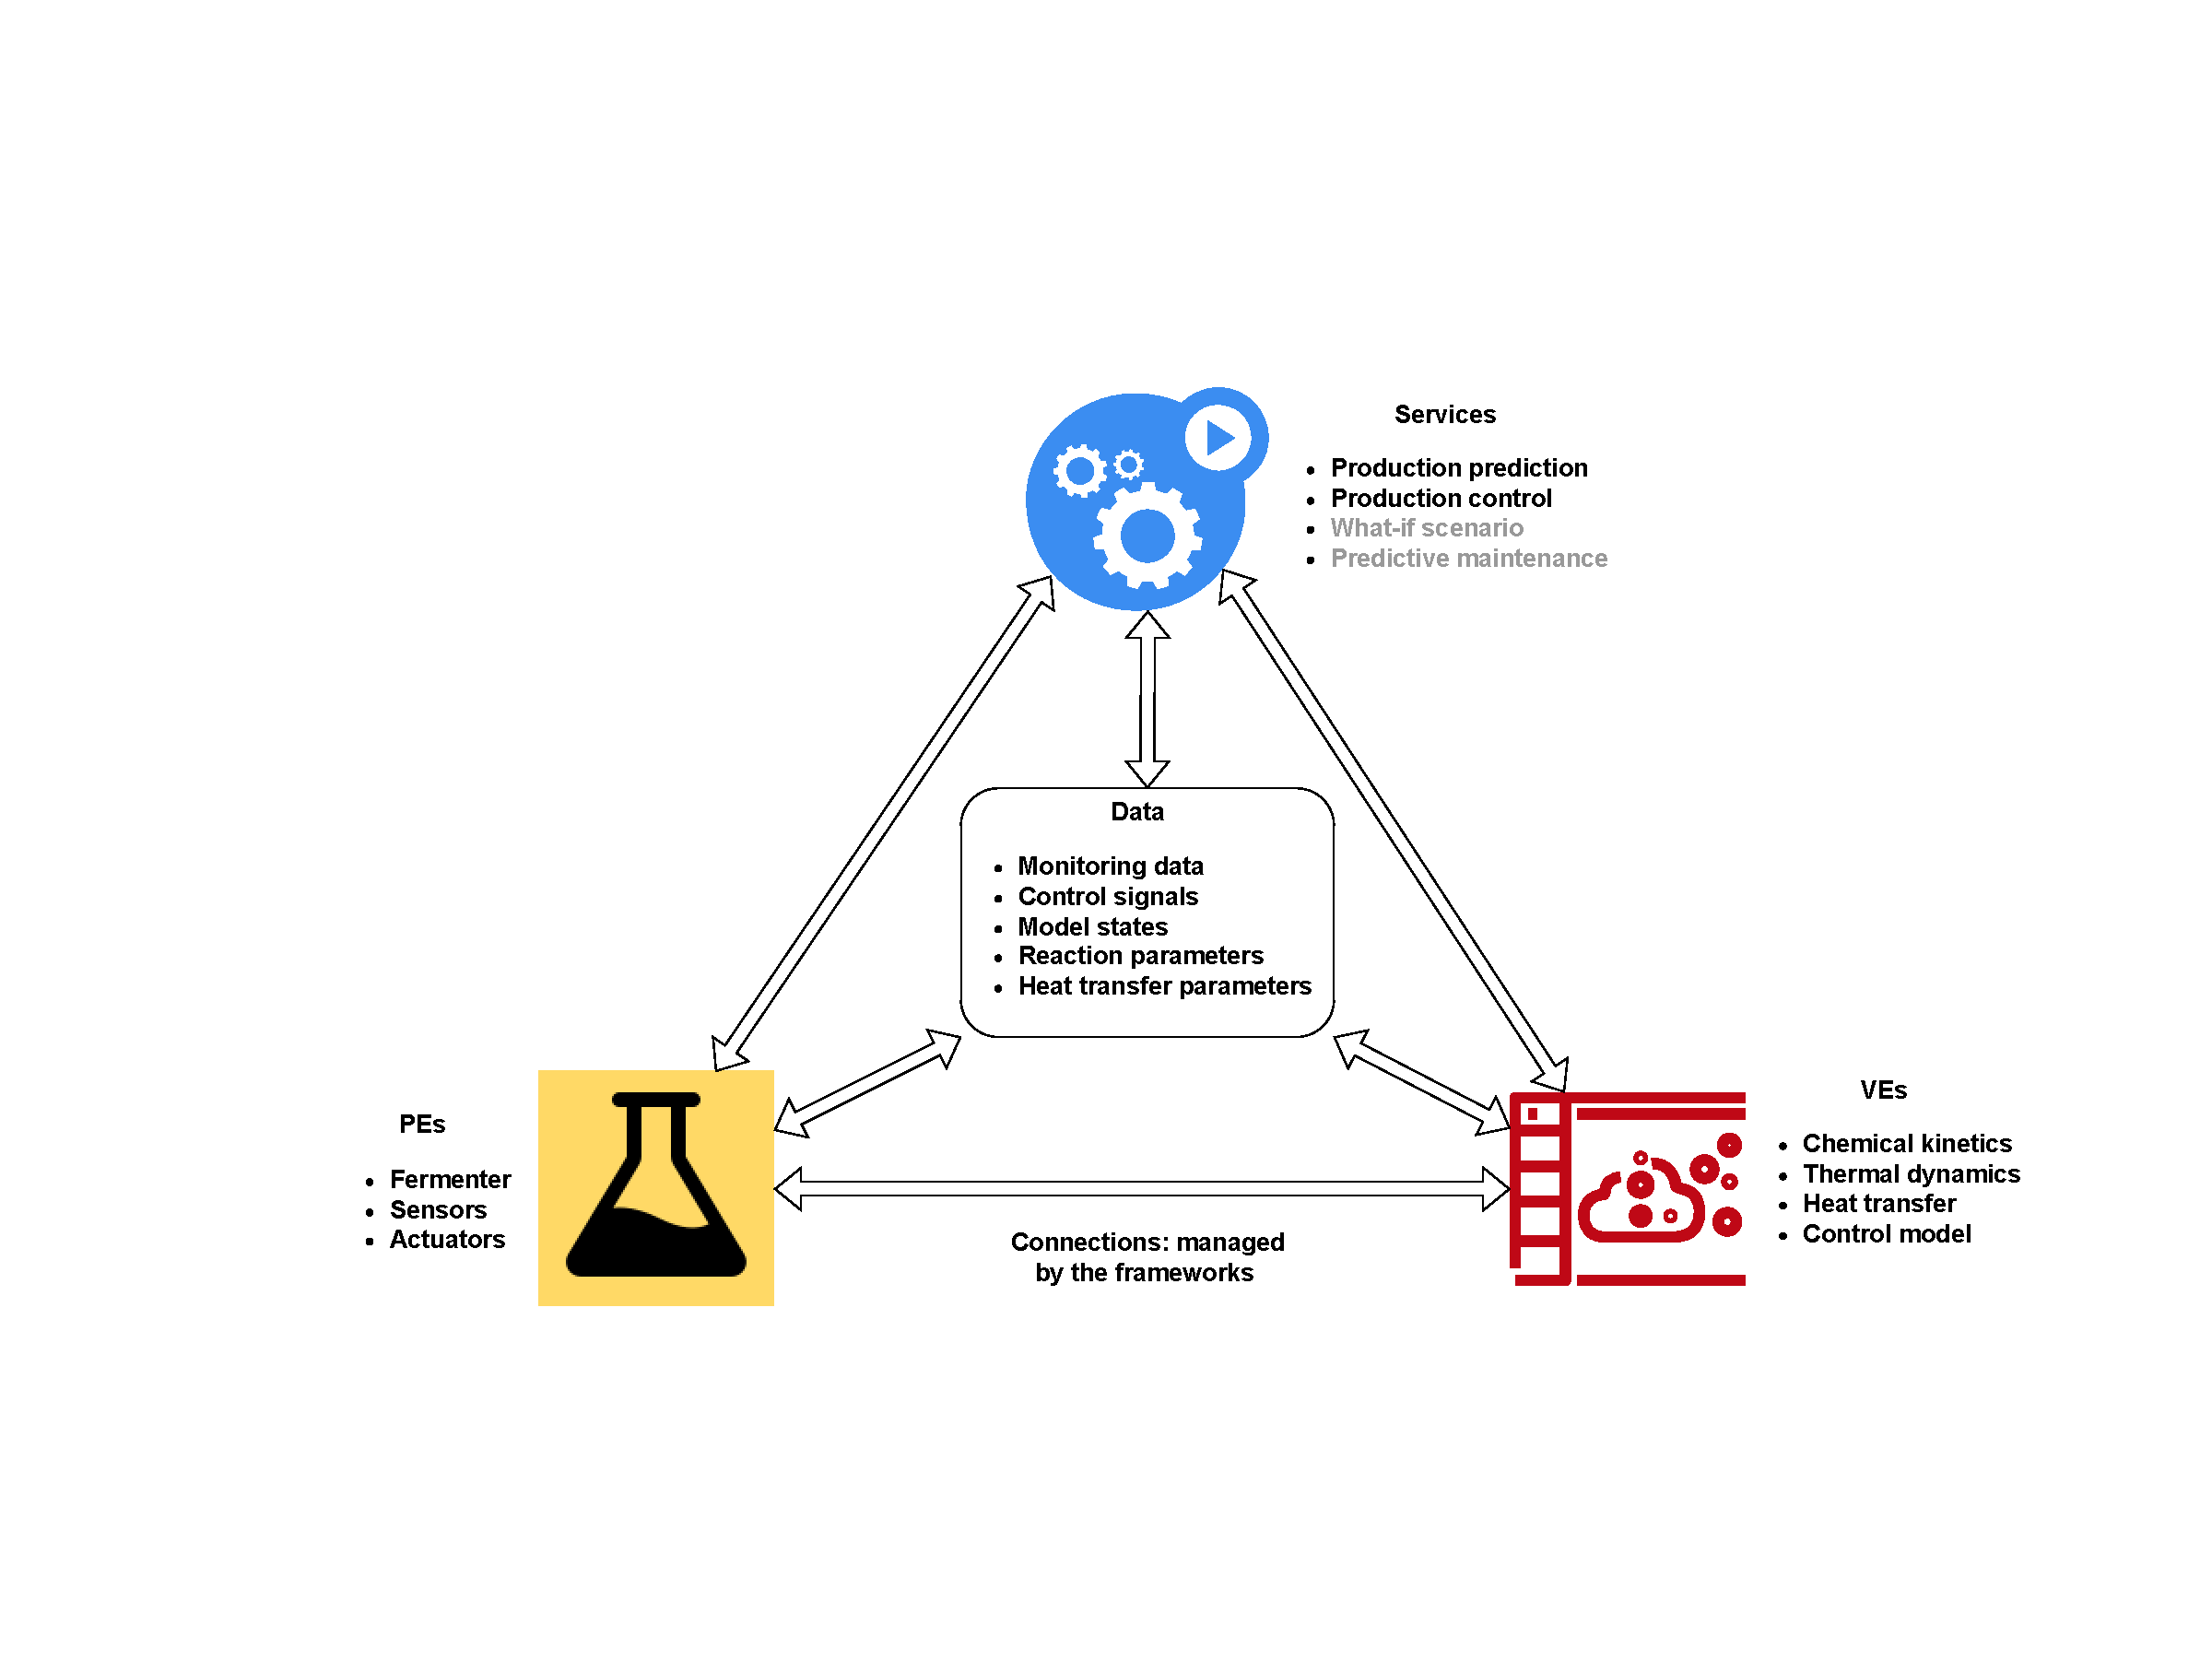
\includegraphics[scale=0.45]{figures/brewery5d.pdf}
  \caption{5D view of the microbrewery DT}
  \label{fig:brewery5d}
\end{figure}

The high level architecture is described using the 5D view (see also Section \ref{sec:overview}), illustrated in Figure \ref{fig:brewery5d}.

\begin{itemize}
  \item \textbf{PEs}: The \textit{fermenter} (also known as bioreactor) is the vessel that holds the wort---the liquid extracted from the mashing process during the brewing of beer. The sensors monitor the temperatures---both inside the fermenter and from the environment, the ambient humidity, and the gravity in the fermenter. The \textit{actuator} is a water pump that can influence the temperature in the system. Appendix \ref{apd:workbench} provides further details of the workbench setup.

  \item \textbf{VEs}: The \textit{chemical kinetics model} is a dynamic model that computes alcohol and yeast concentrations. The \textit{thermal dynamics model} calculates the amount of heat being generated in the system. The \textit{heat transfer model} predicts the future wort temperature. Finally the \textit{control model} produces commands for the actuator in order to alter the temperature to a target value.
  
  \item \textbf{Services}:
  	\begin{itemize}
  	\item \textbf{Production prediction (S1)}: predict the properties of end-product and whether its quantity and quality will meet the demand based on the given materials and resources. 

  	\item \textbf{Production control (S2)}: organize the production schedules and regulate the process such that the utilization of resources is optimized.
  	
  	\item \textbf{What-if scenarios (S3)}: create a hypothetical situation and predict its effect on the production in order to generate variants of the production schedule.
  	
\item \textbf{Predictive maintenance (S4)}: use the data stream from the plant and physical-based modelling to generate a prognosis of the remaining lifetime of plant components.
	\end{itemize}
	
	In order to assess the services and understand the key actors and stakeholders, it is important to recognize their respective phases in the lifecycle. Figure \ref{fig:lifecycle} shows a four-phase lifecycle view \cite{Liu2021} from an industrial perspective and where each proposed service belongs in the cycle.
	\begin{figure}[hbt!]
		\centering
		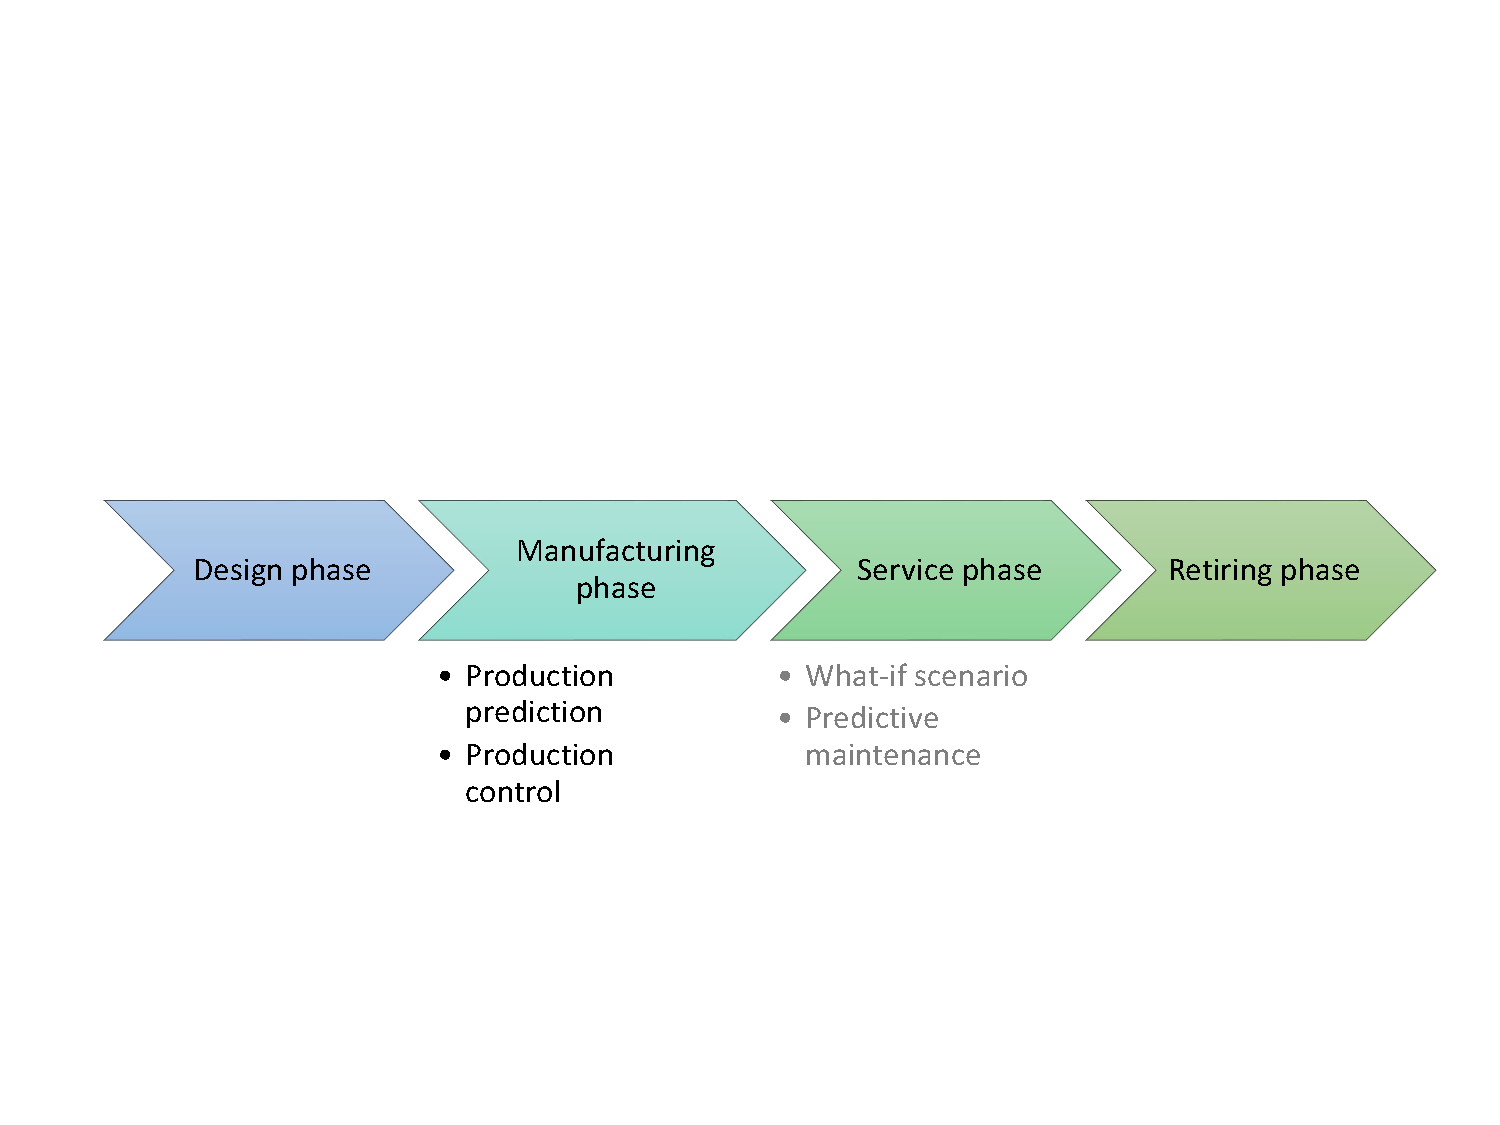
\includegraphics[scale=0.5]{figures/lifecycle.pdf}
		\caption{Services of microbrewery DT in different product lifecycle phases}
		\label{fig:lifecycle}
	\end{figure}
	
The \textit{design phase} encompasses the designs of product, process, and plant, in increasing order of scale. The \textit{manufacturing phase} concerns goods production, and the internal logistical affairs involved. \textbf{S1} and \textbf{S2} primarily concern the questions of production quantity as well as the strategies to optimize the quantity. Therefore, they are considered to be in the manufacturing phase. The \textit{service phase} includes external logistics, user experiences; the detection of anomalies, and repairs. \textbf{S3} and \textbf{S4} fall under this category. In the \textit{retiring phase}, decommissioning of the product is dealt with. Valuable data and parts can be obtained from this recycling action so as to improve the future lifecycles.

Due to the stringent timeline, we only implement \textbf{S1} and \textbf{S2} in this project, reason being that they are considered essential for the brewery operations, and also because \textbf{S3} and \textbf{S4} are, to a considerable extent, based upon the functionalities of the first two services. Nevertheless, we discuss some preliminary designs of \textbf{S3} and \textbf{S4} in the Future work section (Section \ref{sec:futurework}).

  \item \textbf{Data}: The monitoring data are directed from the PEs, and the control signals are directed toward the PE. In the VE space, the \textit{reaction parameters} depend on the chosen beer flavor. The \textit{heat transfer parameters} are the static function of the physical attributes of the fermenter. The remaining data from the VEs are generally denoted as model states. 
   
  \item \textbf{Connections}: They are managed in different fashions by the selected frameworks. More about them will discussed in the later Section \ref{sec:selframe} and Chapter \ref{ch:implementation}.

\end{itemize}

\section{System context description}
Using SysML syntax, the system context is described in Figure \ref{fig:systemcontext} below. The physical components, such as \textbf{Fermenter}, \textbf{Sensors}, and \textbf{WaterPump} are given as the parts of project context.

\begin{itemize}
\item \textbf{DigitalBrewery} is the representation of the microbrewery DT. It makes associations with the other blocks which represent the components of the DT.

\item \textbf{PredictionSystem} and \textbf{ControlSystem} are the embodiments of the VE models and the corresponding services.

\item \textbf{DataManagement} corresponds to the components that manage the storage and the transferring of data.

\item \textbf{I\&O\_Framework} corresponds to the selected integration and orchestration framework in this project. 

\end{itemize}

\begin{figure}[hbt!]
  \centering
  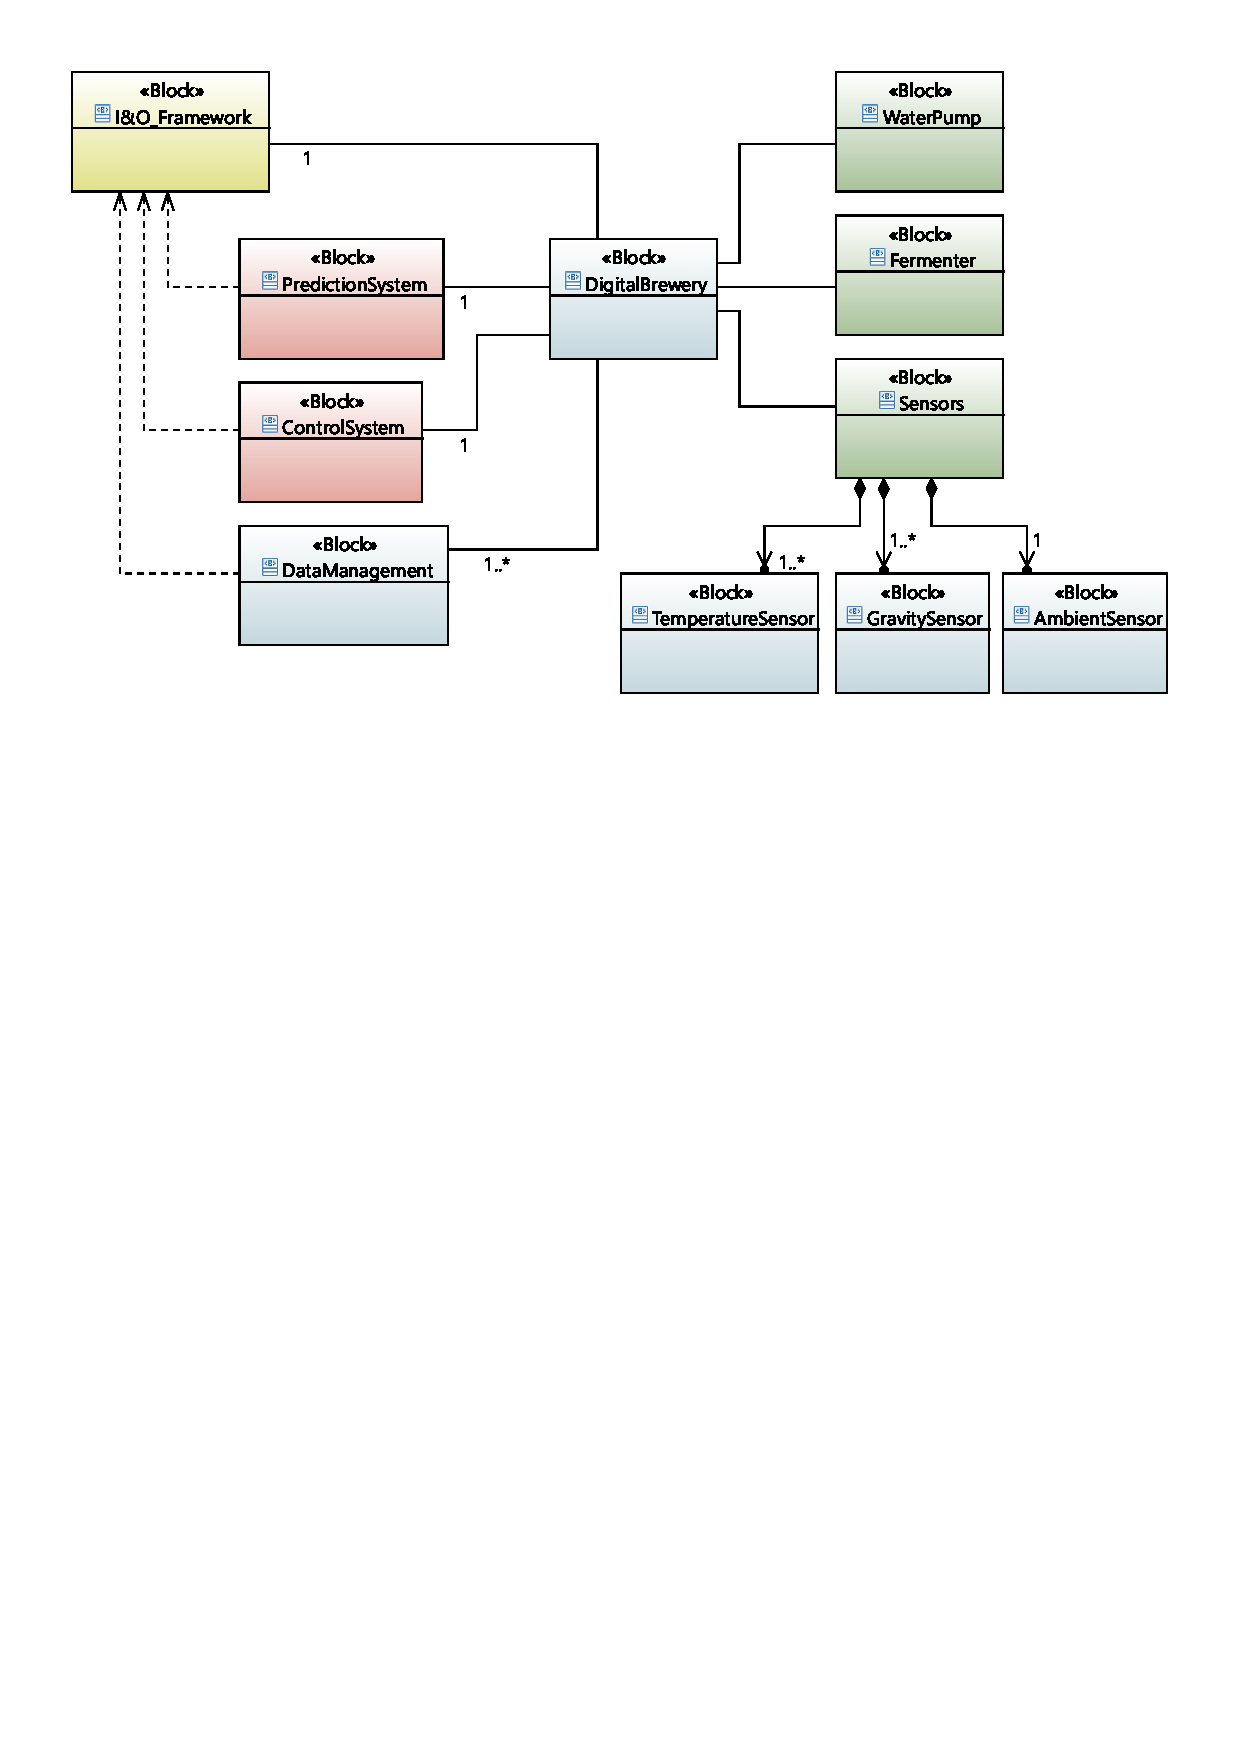
\includegraphics[scale=0.75]{figures/systemcontext.pdf}
  \caption[System context of the brewery DT]{System context of the brewery DT. The PE components are denoted in green. The blocks in red color encompass the services and the process models in VEs. The yellow block represents the integration and orchestration framework.}
  \label{fig:systemcontext}
\end{figure}

\newpage
\section{Requirements identification}\label{ch:req}
\subsubsection{Derivation rationale}
First we highlight a collection of characteristics aligning with the integration and orchestration theme. This collection is gathered based on the high frequency of occurrences found across the literature of bioprocessing DTs. The findings are elicited in Table \ref{tab:iotopics}. Later in this section, these characteristics will become the basis for deriving the requirements of the DT services.

\begin{table}[hbt!]
\centering
\begin{tabular}{|l|l|}
\hline
\textbf{ID} & \textbf{Integration} \\ \hline           
I1 & Configurability of parameters and time advancement \\ \hline
I2 & Automated code/data generation for integration \\ \hline
I3 & Data exchange consistency \\ \hline
I4 & Modularity \\ \hline    
I5 & Ontology checking \\ \hline
\hline                     
   & \textbf{Orchestration} \\ \hline
O1 & Control workflow and execution sequence \\ \hline
O2 & Managing mixed fidelity/granularity \\ \hline
\end{tabular}
\caption{Highlighted characteristics of integration and orchestration}
\label{tab:iotopics}
\end{table}

\textbf{I1} can be further broken down to two parts. First is the adjustability of initialization of the subsystems. As Tolksdorf et al. \cite{Tolksdorf2016} point out, upon the convergence of sub-models into one flowsheet, process engineers often face the challenge of guessing sensible initial values as the sub-models no longer are transparent to them, and a poor guess can easily lead to underperforming models. Therefore, it is argued that the accessibility to critical parameters throughout the whole process is essential to integration. The second part is related to the importance of time step management. In \cite{Neema2014}, the researchers experiment with varying execution step-sizes for a vehicle DT, showing that to a certain degree, distributed components can be ran with different clock rates and still produce matching results. The ability to parameterize time advancement extends flexibility in the platform under design.

\textbf{I2} refers to the required automation to combine models in order to reduce human errors. As chemical process optimizations are rarely accomplished by one single program, manually interfacing multiple simulation packages becomes impractical as soon as the system grows large \cite{Krone2020}. A systematic method to generate ``glue code' including data adaptation is an ideal solution. In practice, we tend to consider a hybrid scheme with varying levels of automation as realistic, as full automation could be too difficult to achieve.

\textbf{I3} suggests in the case when a variable is transferred from one model to another, it shall retain its structure and its dependency relation with other objects. An important implication of this property occurs when several solvers are working on shared data. If information about algebraic dependencies between outputs and inputs is supplied, the importing tool is able to detect and handle algebraic loops automatically \cite{Blochwitz2011}.
 
In \textbf{I4} the modularity property implies not only the plug-and-play accessibility of the models, but also the support for templates---static reuse of resources---and instances---dynamic reuse of resources. Actor-oriented design orthogonalizes component definition and component composition, allowing them to be considered independently \cite{Lee2004}. It promotes modularity which in turn reduces the associated design costs. 

\textbf{I5} considers ontologies. An ontology is the  explicit organization of constituent concepts and the relations between those concepts. More specifically, an ontology can help to express the intended use of a model. In \cite{Ptolemaeus2014}, it is indicated that errors may arise from ontology inconsistencies, as illustrated in Figure \ref{fig:o2ont}.

\begin{figure}[hbt!]
  \centering
  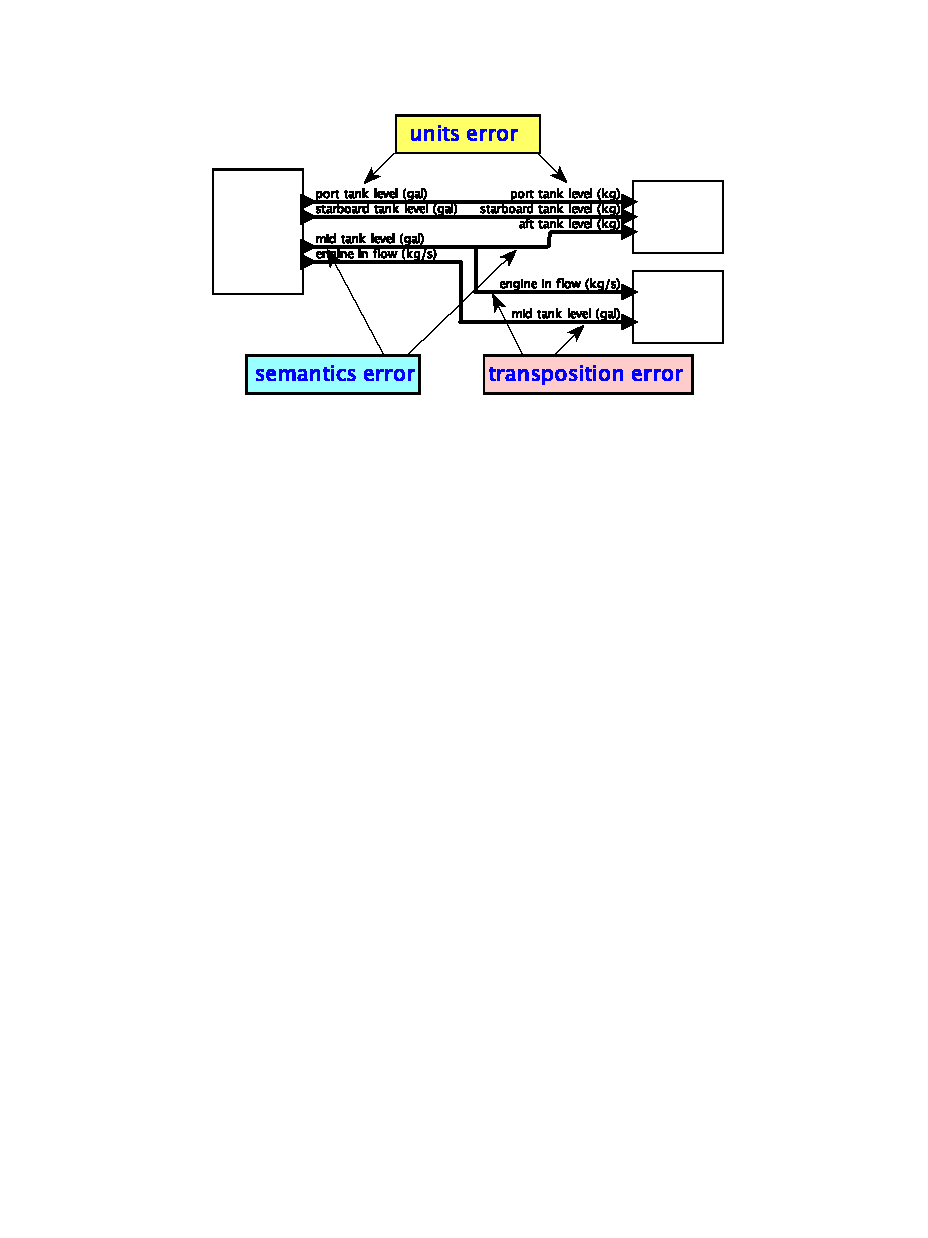
\includegraphics[scale=0.9]{figures/o2ont.pdf}
  \caption[Errors that can be detected by ontology checking]{Errors that can be detected by ontology checking  \cite{Ptolemaeus2014}}
  \label{fig:o2ont}
\end{figure}

\newpage
\textbf{O1} reinforces the importance of effective scheduling. One of the key factors that influences the workflow between models is coupling \cite{Karolius2018}, that is, how tightly are models intertwined with one another. A loose coupling relation generally requires less complex schedules. One may use strategies such as using an external framework to de-couple a pair of inherently coupled models. Other considerations, such as atomicity, might be required should there be concurrent processes.

\textbf{O2} concerns time synchronization and convergence across different models. For instance, merging discrete and continuous time granularities by techniques of sampling and quantization; another example, signaling between time and untimed models. In the case of FMI, an event instant may be driven by a predefined time event or at the transition of state event indicators \cite{Blochwitz2011}. This is to allow numerical robustness, and is a part of the FMI feature which is known as ``hybrid ODE".

The mixed fidelity of data implies varying levels of accuracy in which models' data to quantify the system. This property is often correlated to the computational intensity used by the models. The discrepancy may be solved by data manipulation techniques such as interpolating missing data or sampling out redundant data.

\subsubsection{Production Prediction (S1) Requirements}
The requirements for Production Prediction service are shown in Table \ref{tab:s1req}. The rightmost column indicates the relevant integration and orchestration characteristics.

In addition to requirements, we elicit a set of KPIs in Table \ref{tab:s1kpi}, whose purpose is to verify the effectiveness of the DT regarding how it satisfies the requirements. In principle, each KPI should be a measurable metric that reflects a certain aspect of system performance or non-functional quality. The KPIs are defined in relation to the specific requirements they address.

\begin{table}[hbt!]
\centering
\begin{tabularx}{\textwidth}{|p{1cm}|X|p{2.5cm}|}
\hline
\multicolumn{3}{|c|}{\textbf{Requirements}} \\
\hline
\textbf{ID} & \textbf{Requirement description} & \textbf{Derived from} \\ 
\hline            
R1 & The model state variables shall be validated with real-time empirical data. & I3, I5, O2 \\ 
\hline
R2 & The operator shall be able to configure the initial model parameters and the model execution scheme. & I1 \\ 
\hline
R3 & The model states shall update automatically based on the latest real-time data. & I2, I3, O1 \\ 
\hline
R4 & The model may be queried for its past states in order to optimize its present parameters. & I1, I4, O1 \\ 
\hline
\end{tabularx}
\caption{S1 requirements}
\label{tab:s1req}
\end{table}

\begin{table}[hbt!]
\centering
\begin{tabularx}{\textwidth}{|p{1cm}|p{2.5cm}|X|p{1.5cm}|}
\hline
\multicolumn{4}{|c|}{\textbf{KPIs}} \\ 
\hline
\textbf{ID} & \textbf{Name} & \textbf{Description} & \textbf{Verifies} \\ 
\hline
KPI1 & Level of automation & What are the manual steps required to support the automation of the validation workflow. & R1, R4 \\ 
\hline
KPI2 & Updating delay & How long does it take to perform model state updates. & R3 \\ 
\hline
KPI3 & Data history & What is the amount of historical data that is available for performing predictions. & R4 \\ 
\hline
KPI4 & Modifiability & What configuration options are accessible for model executions and initial values after startup & R2 \\ 
\hline
\end{tabularx}
\caption{S1 KPIs}
\label{tab:s1kpi}
\end{table}

\subsubsection{Production Control (S2) Requirements}
Table \ref{tab:s2req} and Table \ref{tab:s2kpi} shows the requirements and KPIs respectively for the Production Control service.

\begin{table}[hbt!]
\centering
\begin{tabularx}{\textwidth}{|p{1cm}|X|p{2.5cm}|}
\hline
\multicolumn{3}{|c|}{\textbf{Requirements}} \\
\hline
\textbf{ID} & \textbf{Requirement description} & \textbf{Derived from} \\ 
\hline            
R1 & Model optimization may be triggered on the detected disturbance, time, or plant-wide performance. & I5, O1, O2 \\ 
\hline
R2 & Controller calibration may be triggered on time, or state variables deviation. & I2, I5, O1, O2 \\ 
\hline
R3 & Service shall ensure that the calibrations comply with the controller's desired operating range. & I1, I5, O1 \\ 
\hline 
\end{tabularx}
\caption{S2 requirements}
\label{tab:s2req}
\end{table}

\begin{table}[hbt!]
\begin{tabularx}{\textwidth}{|p{1cm}|p{2cm}|X|p{1.5cm}|}
\hline
\multicolumn{4}{|c|}{\textbf{KPIs}} \\ 
\hline
\textbf{ID} & \textbf{Name} & \textbf{Description} & \textbf{Verifies} \\ 
\hline
KPI1 & Traceability & How accessible is the information which concerns the control-induced transitory behaviors. & R3 \\ 
\hline
KPI2 & Latency & What is the response time of actuator triggering. & R1, R2 \\ 
\hline
\end{tabularx}
\caption{S2 KPIs}
\label{tab:s2kpi}
\end{table}

\section{Use case description}
This section covers the use case description for \textbf{S1} and \textbf{S2}.

Figure \ref{fig:usecase1} illustrates the use case diagram for the \textbf{PredictionSystem}. This is corresponding to S1, Production Prediction service.

\begin{figure}[hbt!]
  \centering
  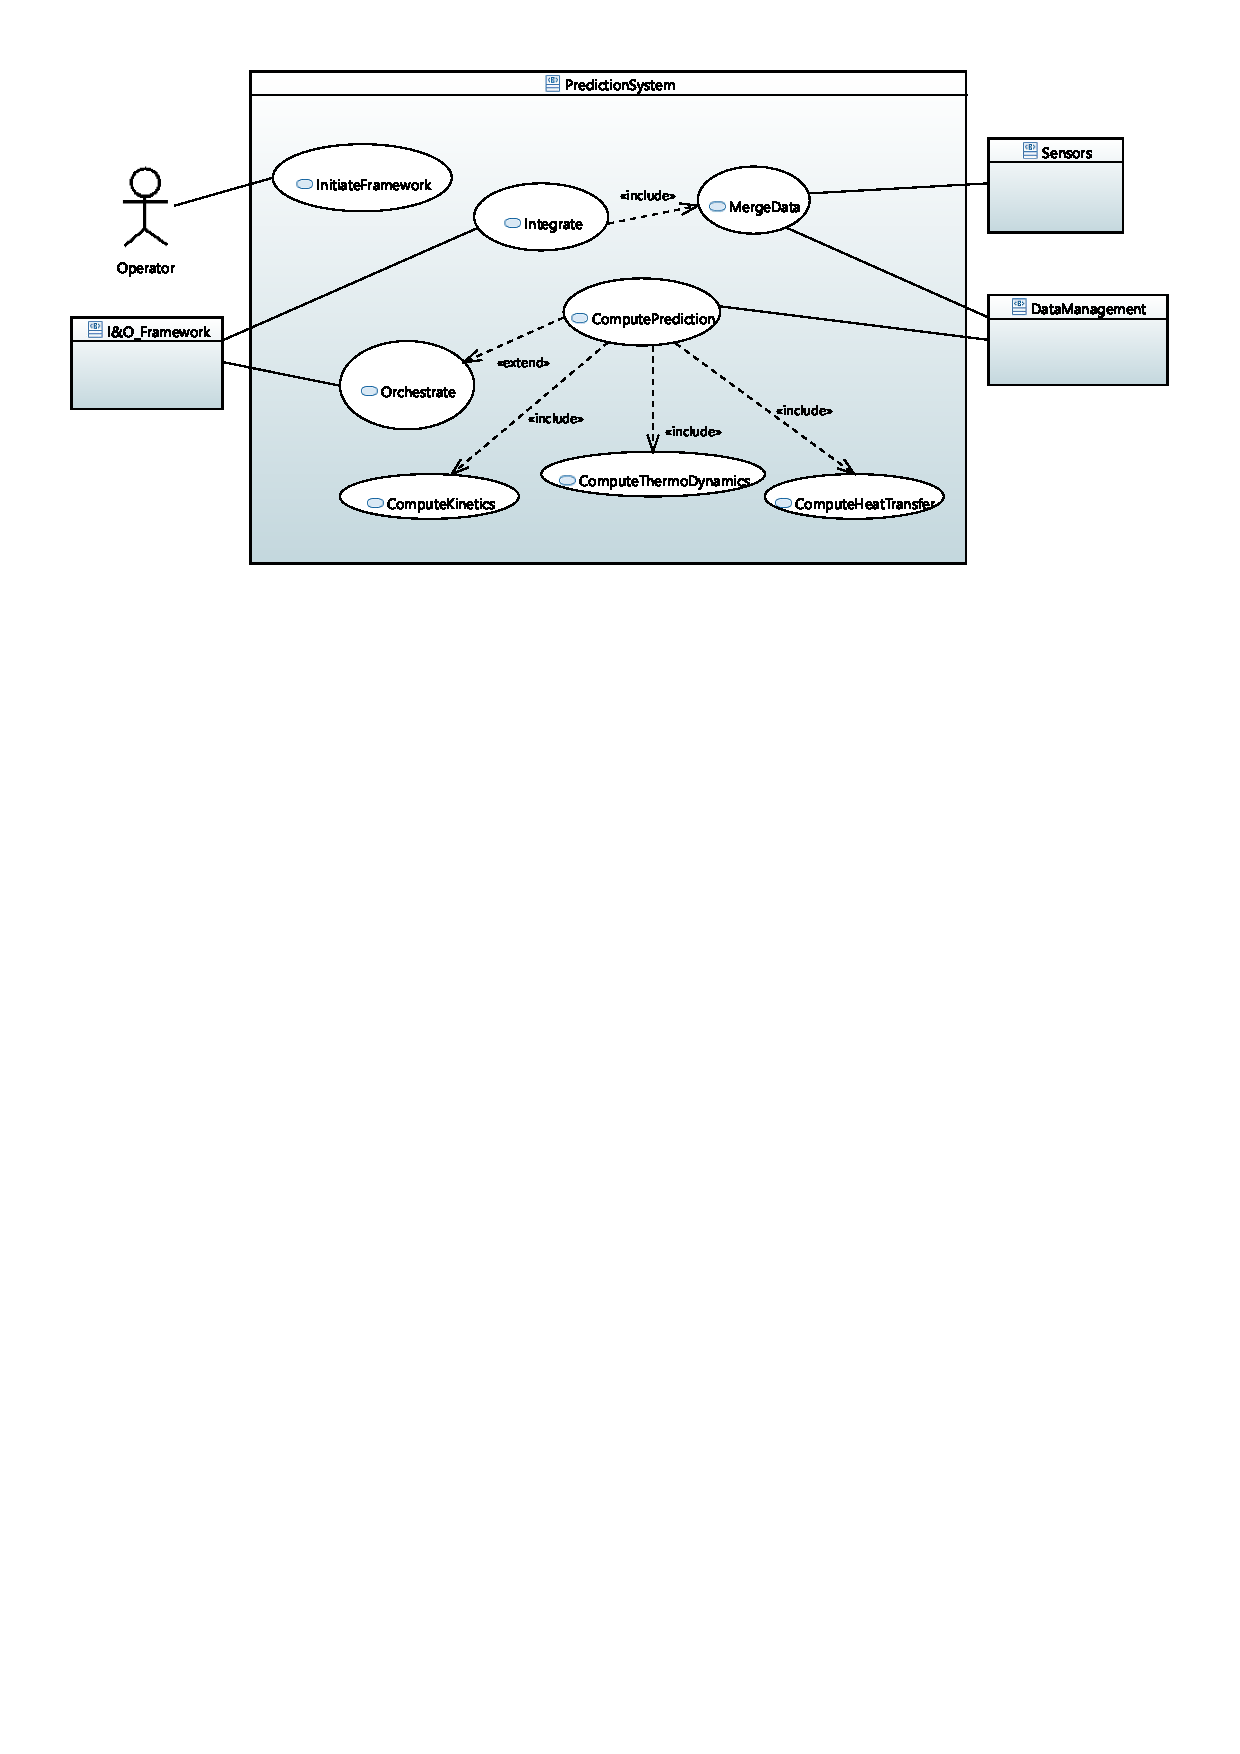
\includegraphics[scale=0.8]{figures/usecase1.pdf}
  \caption{Use cases for S1 scenario}
  \label{fig:usecase1}
\end{figure}

\begin{itemize}
\item In the \textbf{InitiateFramework} use case, \textbf{Operator} accesses the user interface and configures the framework in order to start up the DT.  

\item \textbf{Integrate} manages the data from different sources. It includes \textbf{MergeData} which merges data of the sensors and the model states.

\item \textbf{Orchestrate} manages the scheduling among the models, as well as the validation and updates of the model states.

\item \textbf{ComputePrediction} includes all the calculations in order to generate a prediction value. It includes three use cases that correspond to the VE models of the same name.

\end{itemize}

Figure \ref{fig:usecase2} illustrates the use case diagram for the \textbf{ControlSystem}. This is corresponding to S2, Production Control service.

\begin{figure}[hbt!]
  \centering
  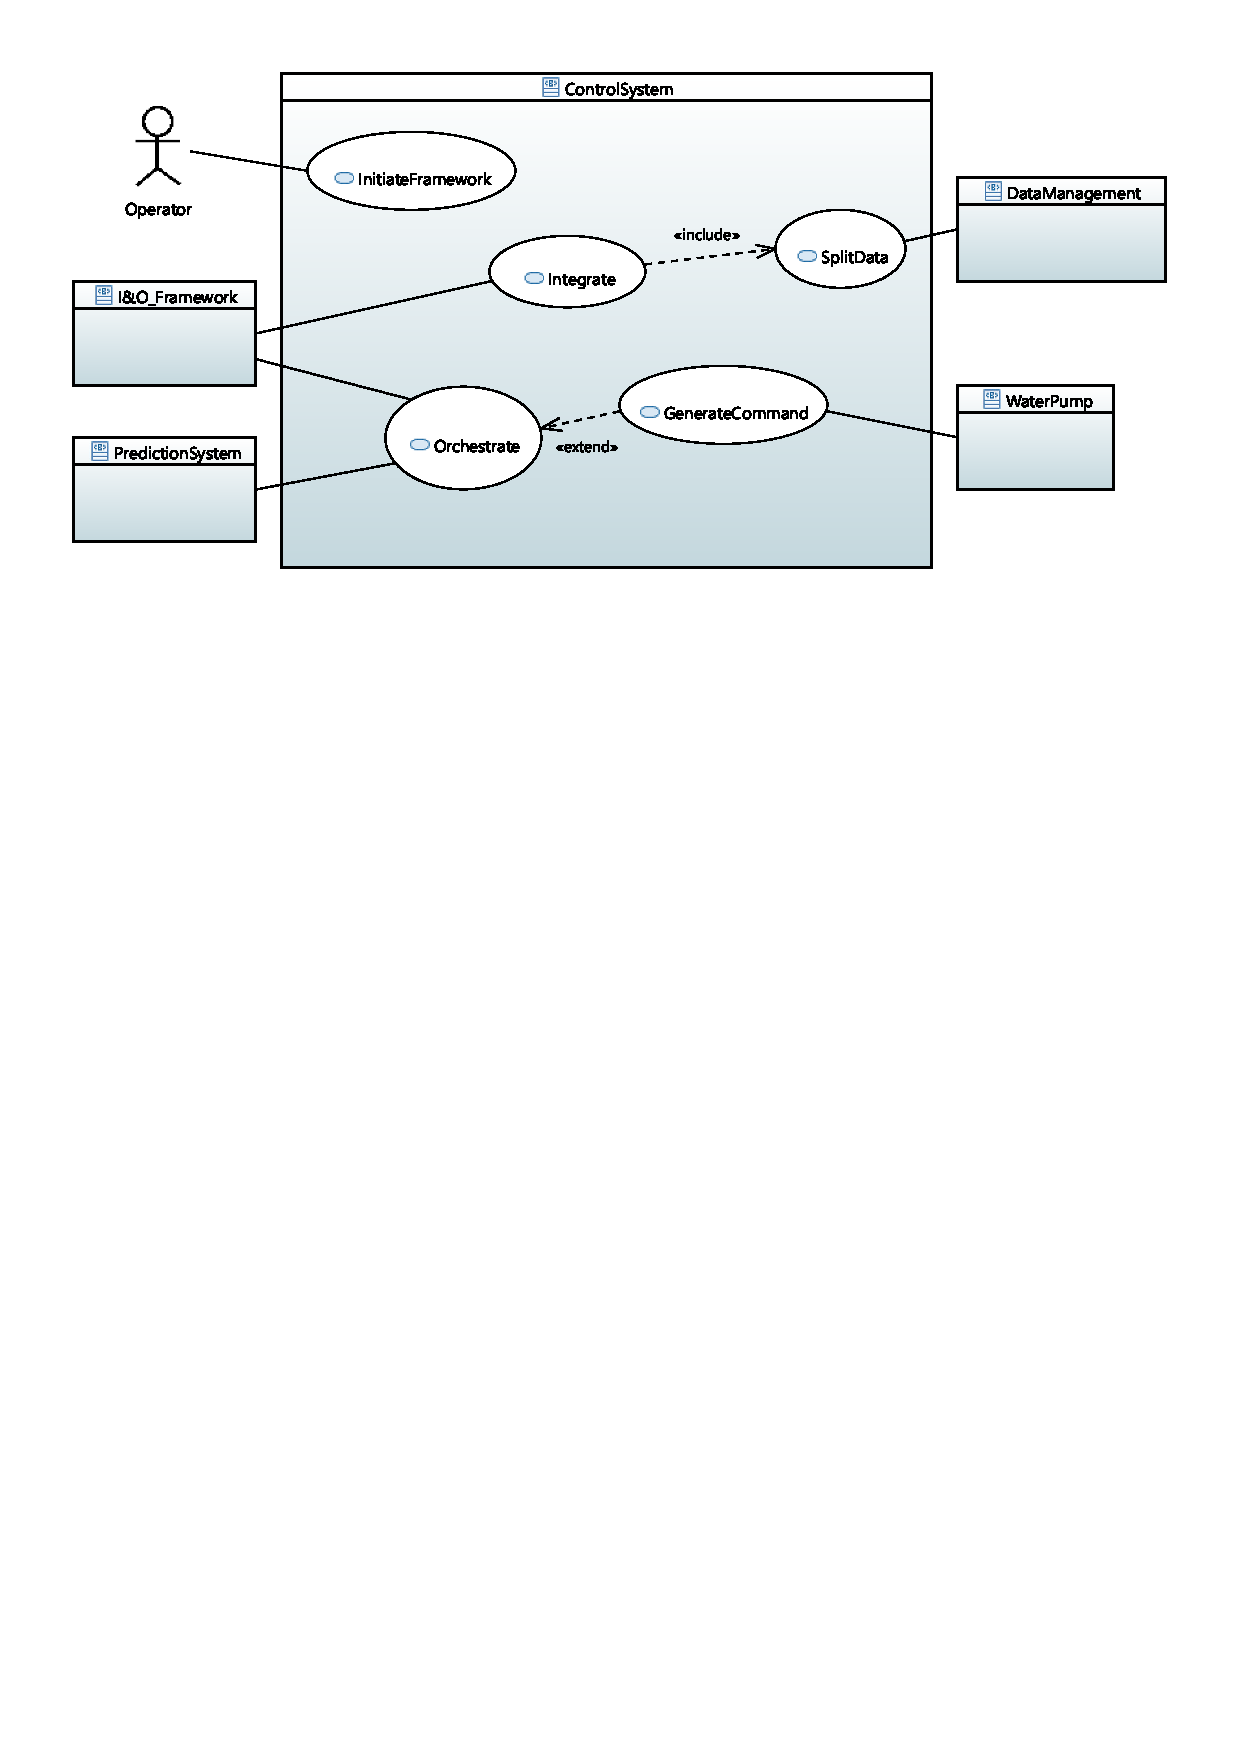
\includegraphics[scale=0.75]{figures/usecase2.pdf}
  \caption{Use cases for S2 scenario}
  \label{fig:usecase2}
\end{figure}

\begin{itemize}
\item \textbf{InitiateFramework}, \textbf{Integrate}, and \textbf{Orchestrate} use cases have the same behaviors as in the S1 scenario.

\item \textbf{SplitData} splits the raw data of control to the right destinations in \textbf{DataManagement}, with the necessary formatting modifications.

\item \textbf{GenerateCommand} uses the control model in VE to generate the control signals to the \textbf{WaterPump}.
\end{itemize}


\section{Selected frameworks} \label{sec:selframe}
This section covers the architecture and workflow of three frameworks, namely, TwinOps, Thingsboard, and Ptolemy II. They are intended for applying integration and orchestration techniques.

These three frameworks are chosen to reflect on the broad spectrum of the software technology sectors, and to highlight the similarity and difference of approaches under the DT context. TwinOps inherits the CI/CD paradigm from DevOps which aims to eliminate the boundary of developments and operations in order to accelerate the software delivery. We argue that this concept can improve the delivery of DT services as well. Thingsboard has its root in the IoT field, which has always regarded the connectivity between ``things" as its core focus. We think this focus can also benefit the connectivity of DT entities. Ptolemy II provides an experimentation platform for CPSes. The management of cyber-objects and physical objects in Ptolemy II is highly applicable to the orchestration and integration of DTs.
 
\subsection{TwinOps} \label{sec:selframe_twop}
The workflow of TwinOps stresses automated transformations, starting at the models in VEs, all the way to the programs running in the PEs. This is also referred as \textit{Model-to-Code-to-Target CI/CD} in the original paper \cite{Hugues2020}. For the feedback direction, the execution traces from PEs are used to validate and update the models, hence closing the pipeline loop. Figure \ref{fig:twinops_workflow} illustrates:

\begin{figure}[hbt!]
  \centering
  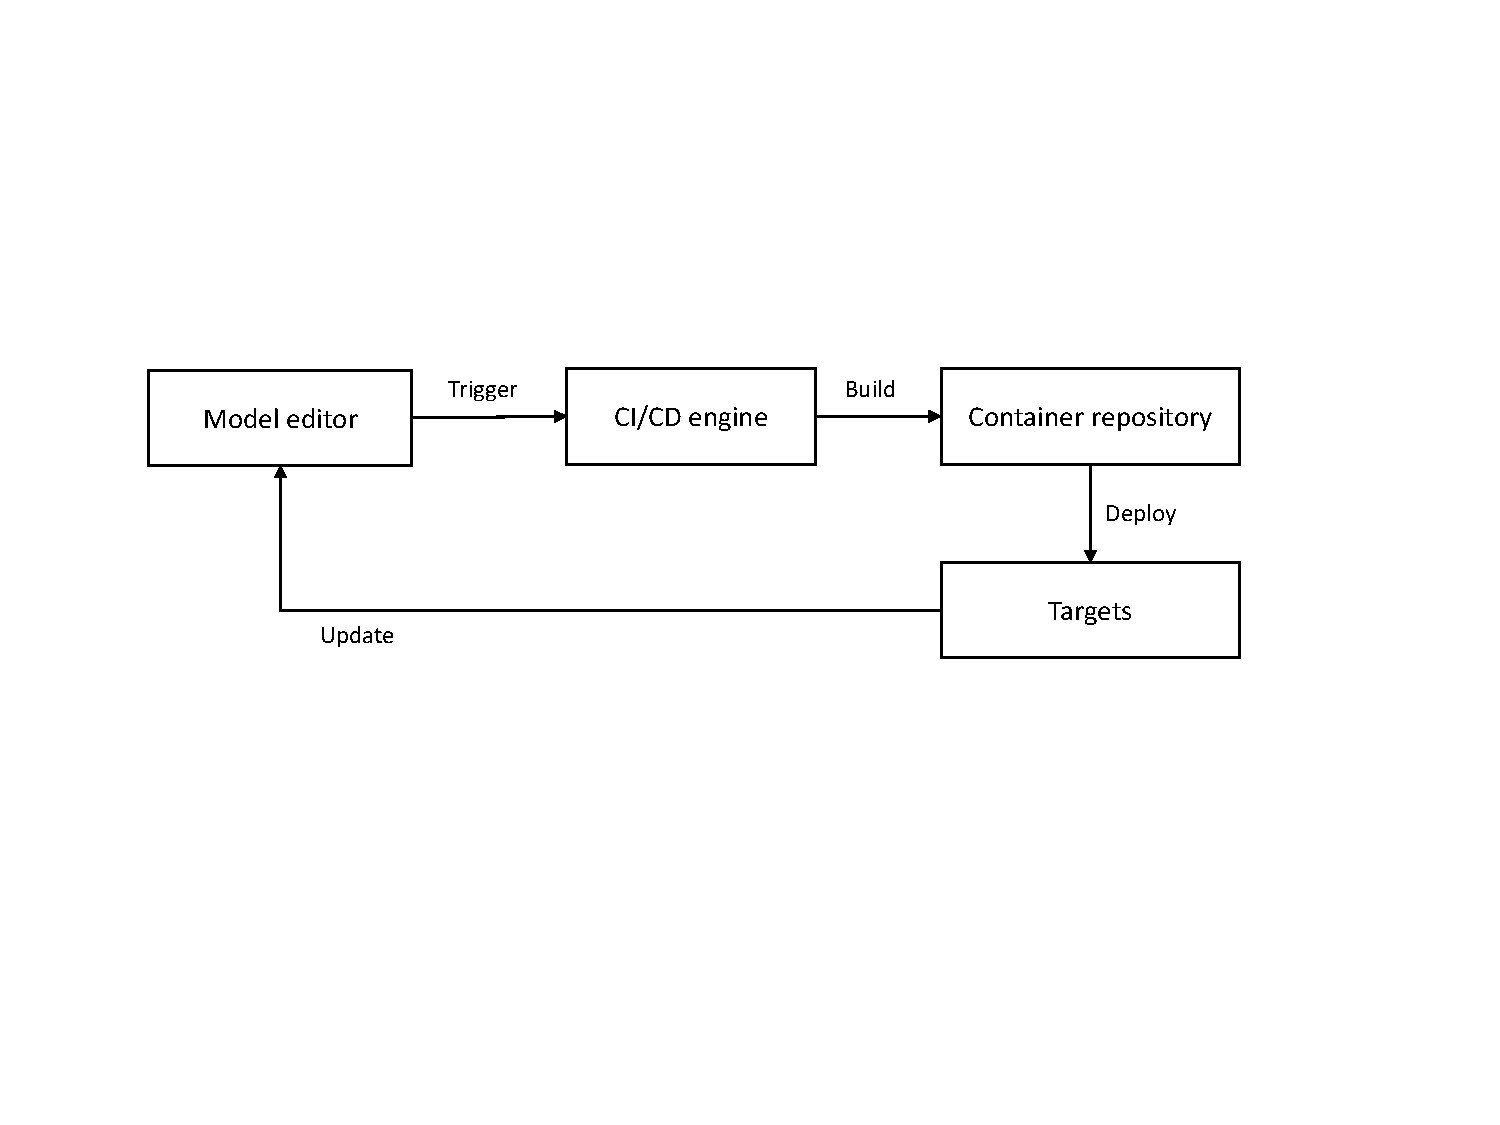
\includegraphics[scale=0.6]{figures/twinops_workflow.pdf}
  \caption{TwinOps workflow}
  \label{fig:twinops_workflow}
\end{figure}

\begin{itemize}

\item \textbf{Model editor}: responsible for building models, drawing the ports topology, and configuring the initial states. 
\item \textbf{CI/CD engine}: integrating the models committed by the previous pipeline stage; validating the models with real-world data; building the containerized image upon passing of all integration tests.
\item \textbf{Container repository}: a hub which stores numerous iterations of models' artifacts---such as the generated code---for the targets. This allows the targets to use the latest codes or rollback to previous versions. It is presumed that the targets in DTs run on diverse platforms (e.g., x86, x64, or ARM), hence the container infrastructure helps to distribute the artifacts efficiently.
\item \textbf{Targets}: a collection of PEs, which can pull the updated program from the repository, as well as produce data analytics which are used for the services.

\end{itemize}

It is important to recognize that the TwinOps framework is not bound to specific technologies or tools. The DT operator has the liberty to choose the collection of building blocks which fits best to the use case, as long as this choice is able to fulfill the workflow outlined in Figure \ref{fig:twinops_workflow}. The toolset implemented in the microbrewery DT will be described in Subsection \ref{sec:s1twop}.

\subsection{ThingsBoard} \label{sec:selframe_tb}
ThingsBoard \cite{Thingsboard} project supports M2M-style network. Essentially, it is an open-source platform that enables rapid development, management, and scaling of IoT projects. The key concepts of ThingsBoard are that the user can provision devices and assets; define relations between them and build rule chains that handle the event processing across the relations. From these features, we see the potentials in supporting the integration and orchestration of our DT. Figure \ref{fig:thingsboard_workflow} illustrates the workflow.

\begin{figure}[hbt!]
  \centering
  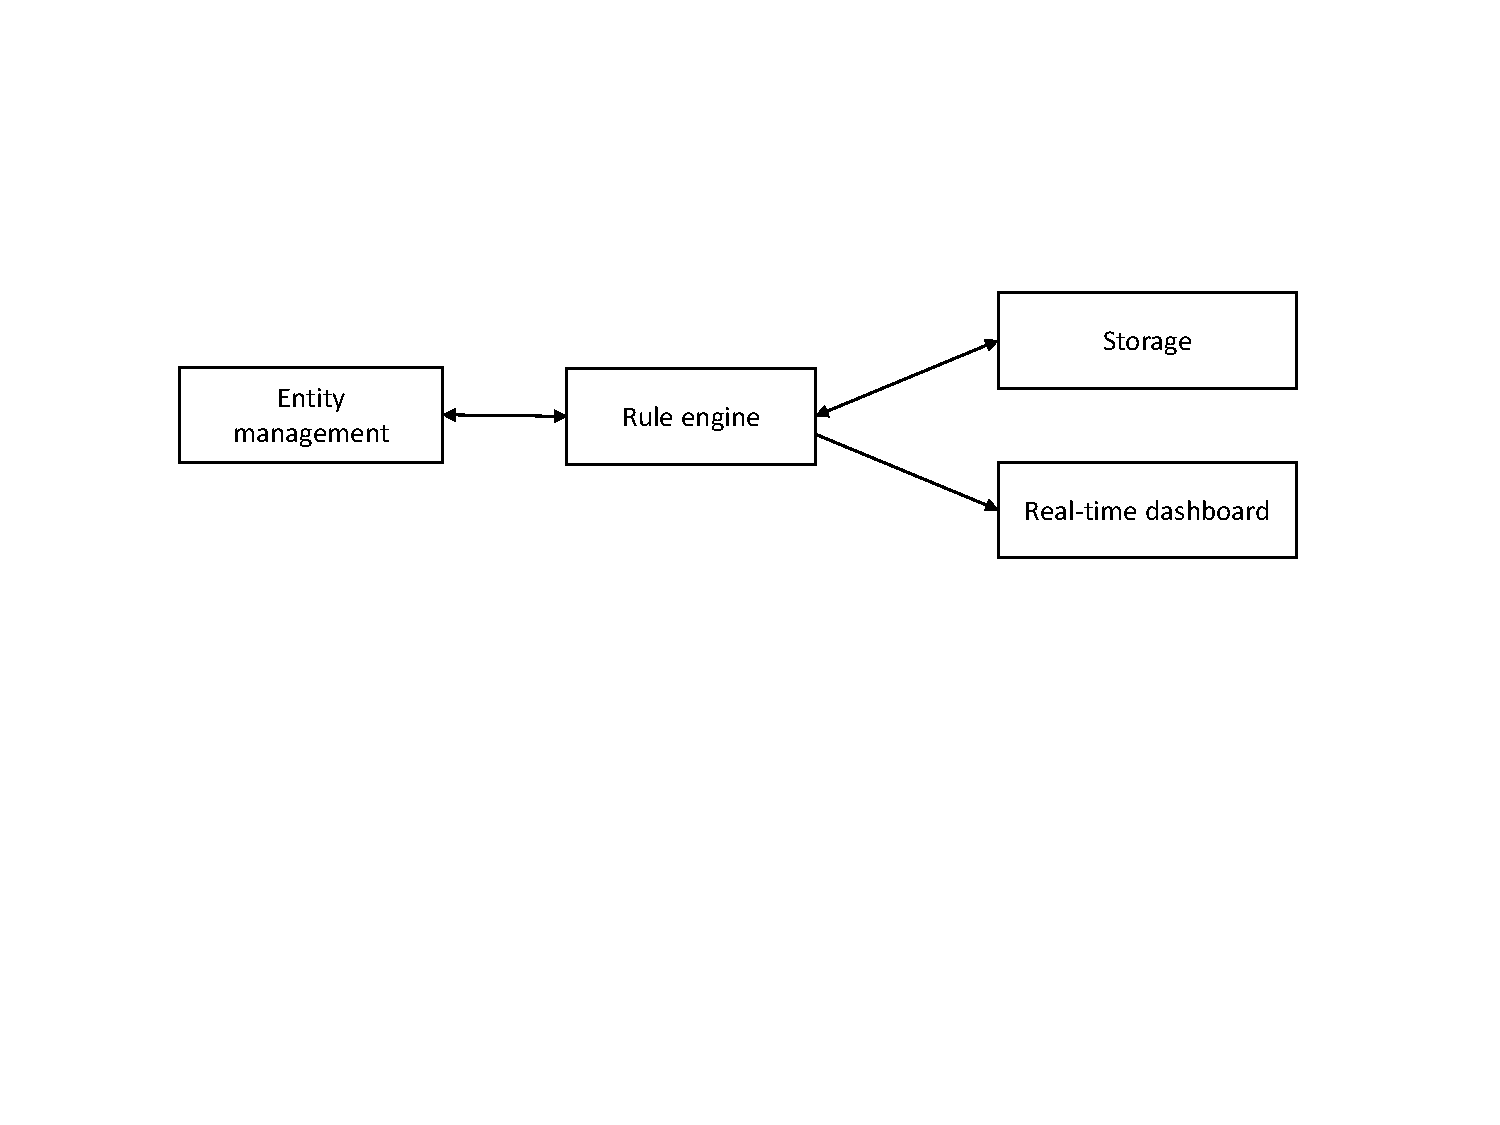
\includegraphics[scale=0.6]{figures/thingsboard_workflow.pdf}
  \caption[ThingsBoard workflow]{ThingsBoard workflow. The arrows represent the direction in which each stage could make modifications to the other stages}
  \label{fig:thingsboard_workflow}
\end{figure}

\begin{itemize}
\item \textbf{Entity management}: this is the first step where the user should define all the involved entities and their relations. There are two main entity types. \textit{Device} entity type refers to the basic unit that transmit and receive messages. The \textit{Asset} entity is an abstract type that can form logical grouping of \textit{devices} or other \textit{assets} via \textit{relations}. Commonly used \textit{relations} are ``contains", ``manages", etc.

\item \textbf{Rule engine}: refers to the event-based \textit{rule chains} which are customized by the user. A rule chain consists of connected \textit{rule nodes} which represent functions or conditions. There are built-in node type such as ``filter" or ``transform", etc. The user can also define their own nodes using JavaScript. When a message arrives from the entities the rule engine will produce the corresponding actions based on the \textit{rule chains} and the \textit{relations} which have been given in the entity management stage. As an example, a ``smart building" could impose crowd traffic monitoring using \textit{rule chains} to broadcast the readings of the passengers counter---a \textit{device}---in one elevator to all the other elevators which the building---\textit{an asset}---``contains".

\item \textbf{Storage}: ThingsBoard supports in-memory storage itself, or one can use the data the supported external space, e.g.,  cloud-based.

\item \textbf{Real-time dashboard}: this is related to the user experience and the user interface aspects. The operator can add \textit{widgets} in the dashboard to reflect the events happening in the rule engine in the forms of chart, table or various other visualizations.

\end{itemize}

There are a couple of underlying services called \textit{ThingsBoard Core} and  \textit{ThingsBoard Transports} that basically handle the M2M networking on the platform. They provide communication protocol stacks and account for maintaining the connectivity states. Consequently, they greatly influence system performance. Because these two are background processes, they are omitted in the workflow shown in Figure \ref{fig:thingsboard_workflow}.

\subsection{Ptolemy II}
In Subsection \ref{sec:orch} we have briefly described Ptolemy II from the perspective of actor-oriented model. Here we look at Ptolemy II from the software architecture angle. We aim to utilize it as a DT framework.

The official documentation \cite{Ptolemaeus2014} presents a meta model that describes the Ptolemy II software architecture, as seen in Figure \ref{fig:pt2meta}. Below are some important highlights of the figure:

\begin{itemize}
\item Every component in a Ptolemy II model is an instance of the \texttt{NamedObj} class. There are four subclasses of \texttt{NamedObj}. These are \texttt{Attribute}, \texttt{Entity}, \texttt{Port}, and \texttt{Relation} respectively.
\item \texttt{Relation} class represents communication path between the instances of \texttt{Entity}. 
\item \texttt{Port} class has many-to-many links to \texttt{Relation}, and it also hosts the \texttt{Receiver} interface that implements methods relating to data communication. Together they can be used to manage the models integration. 

\item Implemented by \texttt{Director}, the \texttt{Executable} interface contains methods that orchestrate the modeling progressions. In other words, the interface coordinates the iterations among actors based on the rules of the selected MoC.
\end{itemize}

\begin{figure}[hbt!]
  \centering
  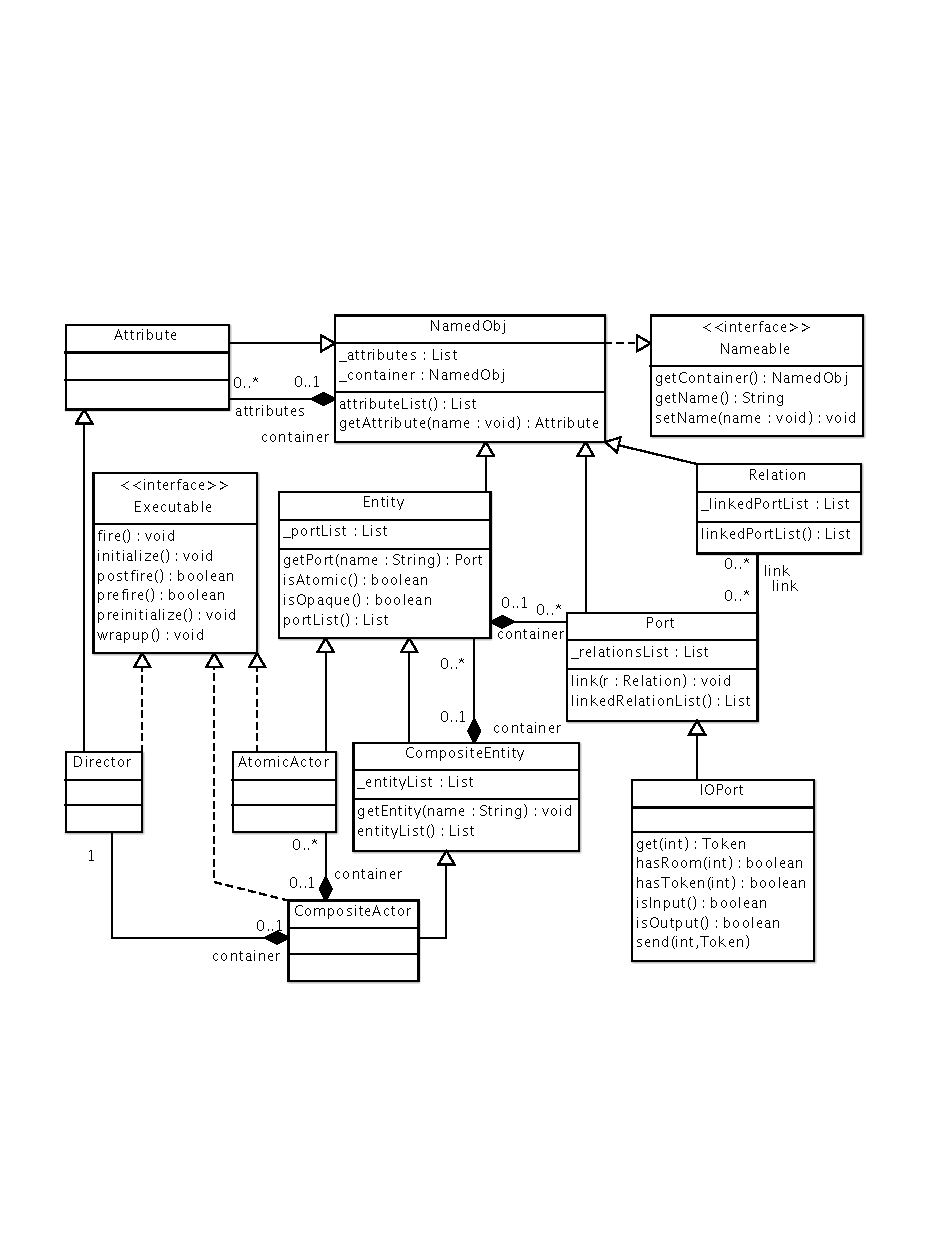
\includegraphics[scale=0.8]{figures/pt2meta.pdf}
  \caption{Meta model of Ptolemy II}
  \label{fig:pt2meta}
\end{figure}

The abstract syntax are implemented as a collection of Java classes and packages. Ptolemy II enables the user to interact with these abstract syntax by the mean of a graphical editing interface, utilizing drag-and-drop actions to accomplish designs.

